\chapter{Momento angular y corchetes de \emph{Poisson}}

	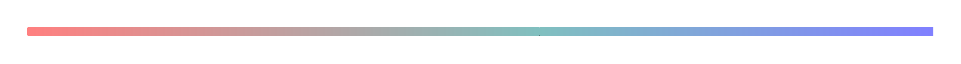
\begin{tikzpicture}
	\fill [left color=red!50, right color=teal!50] (0,0) rectangle (6.5,.1);
	\fill [left color=teal!50, right color=blue!50] (6.5,0) rectangle (11.5,.1);
	\end{tikzpicture}



\vspace{10mm}
\begin{adjustwidth}{50pt}{50pt}
\begin{ejemplo}

Seguimos explorando los corchetes de Poisson y vamos a reformular las ecuaciones de Hamilton en función de ellos y calcularemos también los corchetes de Poisson para el momento angular y veremos cosas muy interesantes.

\end{ejemplo}
\end{adjustwidth}
\vspace{5mm}
\section{Más propiedades del corchete de \emph{Poisson}}
\label{T22CPmasP}

\begin{enumerate}[1.- ]
\vspace{5mm}\item 	Para $\ f(q),\ g(q) \ \to  \{f(q),g(q)\} =  \displaystyle \left( \pdv{f}{q}, \ \pdv{f}{p} \right) \mqty ( 0&1 \\-1&0) \mqty( \displaystyle \pdv{g}{q} \\  \pdv{g}{p} ) = \left( \pdv{f}{q}, \ 0 \right) \mqty(0&1\\-1&0) \mqty( \displaystyle \pdv{g}{q} \\ 0 )= \mqty(f_q & 0) \mqty (0\\-g_q)= 0  \qquad \to \qquad  \subrayado{\boxed{\ \boldsymbol{ \{f(q),g(q)\}\ = \ 0 } \ }} $ 
\vspace{5mm} \item Análogamente, para $\ f(p),\ g(p) \quad \to \quad \subrayado{\boxed{\ \boldsymbol{ \{f(p),g(p)\}\ = \ 0 } \ }} $ 
\vspace{5mm}\item Para $\ f(q),\ g(p) \ \to  \{f(q),g(p)\} =  \displaystyle  \left( \pdv{f}{q}, \ 0 \right) \mqty(0&1\\-1&0) \mqty( \displaystyle  0 \\ \displaystyle \pdv{g}{p} )= \mqty(f_q & 0) \mqty (g_p\\0)= f_q g_p  \qquad \to $

$\to \qquad \subrayado{\boxed{\ \boldsymbol{ \{f(q),g(p)\}\ = \ \displaystyle \pdv{f}{q} \ \pdv{g}{p} } \ }} $ 
\vspace{5mm}\item Generalizando, $\ f(q_1, q_2, \cdots, q_n),\ \ g(p_1, \cdots, p_n) \ \to \ \quad  \subrayado{\boxed{\ \boldsymbol{\{f(q),g(p)\} \ = \  \{f,g\}\ = \  \displaystyle \sum_{s=1}^n \pdv{f}{q_i} \ \pdv{g}{p_i} } \ } }$
\vspace{5mm}\item Para $\ f(p),\ h(q,p) \ \to \ \{f(p),h(q,p)\} = \mqty(0&f_p) \mqty(0&1\\-1&0) \mqty(h_q\\h_p)= \mqty(0&f_p) \mqty(h_p\\-h_q) = -f_ph_q \quad$

$\displaystyle \text{generalizando } \qquad \subrayado{\boxed{\ \boldsymbol{\{f(q),g(q,p)\} \ =  \  \displaystyle - \sum_{s=1}^n \pdv{f}{p_i} \ \pdv{h}{q_i} } \ } }$
\vspace{5mm}\item Corolario-I: $\quad 4)\ Si \ f=q_i \ \to \ \subrayado{\boxed{\ \boldsymbol{ \displaystyle  \{q_i, f_p\} \ = \ \pdv{f}{p} } \ } }$
\vspace{5mm}\item Corolario-II, análogo al anterior: $\quad De \ 5) \ \to \quad \subrayado{\boxed{\ \boldsymbol{ \displaystyle  \{p_i, f_q\} \ = \ -\pdv{f}{q} } \ } }$

\end{enumerate}


\vspace{1cm}
\section{Ecuaciones de \emph{Hamilton} y corchetes de \emph{Poisson}}
?`Para qué sirven estas nuevas propiedades?

Supongamos que tenemos $\ H=T(p_1,\cdots , p_n) +\ + \ V(q_1,\cdots, q_n)\ $ y estamos interesados en calcular:

$\{q_3,H\}=\{q_3,T(p)+V(q)\}=\{q_3,T(p)\}+\cancelto{0}{ \{q_3,V(q)\} }=\{q_3,\ \cancel{p_1}, \cancel{\cdots} + p_i + \cancel{\cdots} + \cancel{p_n} \}=\displaystyle \pdv{T}{p_3}=\pdv{H}{p_3}$

Para $\ \displaystyle \ H=T(p_i)+V(q_i) \ \to \ \ \{q_i,H\}=\pdv{T}{p_i}=\pdv{H}{p_i}$

Del mismo modo, $\displaystyle \ H=T(p_i)+V(q_i) \ \to \ \ \{p_i,H\}=-\pdv{V}{q_i}=-\pdv{H}{q_i}$

Hemos obtenido:
$\quad  \{q_i,H\}=\displaystyle \pdv{H}{p_i} \quad  \begin{matrix} _{Ec H} \\ ^{==} \end{matrix}  \quad \dot q_i  \quad \qquad  \{p_i,H\}=-\displaystyle \pdv{H}{q_i} \quad  \begin{matrix} _{Ec H} \\ ^{==} \end{matrix}  \quad \dot p_i 
$


Luego, podemos formular las ecuaciones de Hamilton en función de los corchetes de Poisson:

\vspace{5mm}
\begin{large}
\begin{myblock}{Ecuaciones de Hamilton en función de los corchetes de Poisson}
$\, $

\begin{equation}
\label{T22EHCP}	
\boldsymbol{
\dot q_i \ = \ \{ q_i, H\} \qquad \qquad \qquad \dot p_i \ = \ \{ p_i, H\} }
\end{equation}

$\, $	
\end{myblock}
\end{large}


\vspace{1cm}
\section{Momento angular y corchete de \emph{Poisson}}
\label{T22CPL}

$\overrightarrow L = (L_1,L_2,L_3) \quad \begin{cases} \ L_1=q_2p_3-q_3p_2 \\ \ L_2=q_3p_1-q_1p_3 \\ \ L_3=q_1q_2 - q_2p_1  \end{cases} \qquad \qquad  \text{ahora } \ \ z=(q_1\ q_2\ \ q_3 \ \ p_1\ p_2\ p_3)^T$

Nos preguntamos qué valdrá $\quad \{q_1,L_1\}= (\ \{f(q),h(q,p)\}\ ) =
\mqty(1\\0\\0 \\ \cdots \\ 0\\0\\0)^T \ \mqty( 0 & \vdots & I \\ \cdots & \cdots & \cdots  \\ -I & \vdots & 0) \mqty( \displaystyle \pdv{L_1}{q_1} \\  \displaystyle \pdv{L_1}{q_2} \\  \displaystyle \pdv{L_1}{q_3} \\ \cdots \\  \displaystyle \pdv{L_1}{p_1} \\  \displaystyle \pdv{L_1}{p_2} \\   \displaystyle \pdv{L_1}{p_3})= 
(1\ 0\ 0\  \vdots \ 0\ 0\ 0)\ \mqty(0\\ -q_3\\q_2\\ \cdots \\ 0\\-p_3 \\p_2)=0$ \hspace{2cm} Análogamente, $\quad \{q_2,L_1\}=(0\ 1\ 0 \ \vdots \ 0\ 0\ 0)\ \mqty(0\\ -q_3\\q_2\\ \cdots \\ 0\\-p_3 \\p_2)=-q_3$

 Y también $\quad \{q_3,L\}=(0\ 0\ 1 \ \vdots \ 0\ 0\ 0)\ \mqty(0\\ -q_3\\q_2\\ \cdots \\ 0\\-p_3 \\p_2)=q_2;\qquad \{p_1,L\}=0;\ \ \{p_2,L\}=-p_3;\ \ \{p_3,L\}=p_2$
 
 Es sencillo comprobar que para $L_2$, con el vector 
 $\mqty( \displaystyle \pdv{L_2}{q_1} \\  \displaystyle \pdv{L_2}{q_2} \\  \displaystyle \pdv{L_2}{q_3} \\ \cdots \\  \displaystyle \pdv{L_2}{p_1} \\  \displaystyle \pdv{L_2}{p_2} \\   \displaystyle \pdv{L_2}{p_3}) = 
 \mqty( -p_3\\0\\p_1\\ \cdots\\ q_3\\0\\-q_1) \quad $  
 
 y para $L_3 \quad  \mqty( \displaystyle \pdv{L_3}{q_1} \\  \displaystyle \pdv{L_3}{q_2} \\  \displaystyle \pdv{L_3}{q_3} \\ \cdots \\  \displaystyle \pdv{L_3}{p_1} \\  \displaystyle \pdv{L_3}{p_2} \\   \displaystyle \pdv{L_3}{p_3}) = 
 \mqty( p_2\\-p_1\\0\\ \cdots\\ -q_2\\q_1\\0) \quad $ se obtienen, respectivamente,
 
 
\hspace{1cm} $\{q_1,L_2\}=q_3 \ \text{cíclico} ;\quad \{q_2,L_2\}=0 \ \text{repetido};\quad \{q_3,L_2\}=q_1 \ \text{cíclico}$

\hspace{1cm} $\{p_1,L_2\}=q_3;\quad \{p_2,L_2\}=0;\quad \{p_3,L_2\}=p1 $

\hspace{1cm} $\{q_1,L_3\}=-q_2 \ \text{no cíclico}; \{q_2,L_3\}=q_1 \ \text{cíclico} \quad \{q_3,L_3\}=0 \ \text{repetido}$

\hspace{1cm} $\{p_1,L_3\}=-p_2;\quad \{p_2,L_3\}=p_1;\quad \{p_3,L_3\}=0$

\vspace{5mm} Todo esto se puede escribir, de forma ordemada, usando el \textbf{\emph{tensor} de Levi-Civita}, $\ \boldsymbol{ \varepsilon_{ijk} }\, ;  \quad  \text{con } \ i,j,k=1,2,3$, tal que si los subíndices están en permutación cíclica, el tensor da $1$. Si la permutación no es cíclica, el tensor de $-1$ y da $0$ si hay algún índice repetido: $\varepsilon_{123}=\varepsilon_{231}=\varepsilon_{312}=1;\ \ \varepsilon_{132}=\varepsilon_{213}=\varepsilon_{321}=-1 ; \ \ \varepsilon_{121}=\varepsilon_{113}=\cdots =0$

\vspace{5mm}
\begin{large}
\begin{myalertblock}{Corchetes de Poisson con el momento angular}

\begin{equation}
\label{T22COL}	
\boldsymbol{
\{\ q_i\ , \ Lj\ \} \ = \ \varepsilon_{ijk}\ q_k
\qquad  \qquad \qquad
\{\ p_i\ , \ Lj\ \} \ = \ \varepsilon_{ijk}\ p_k
}
\end{equation}	
\end{myalertblock}
\end{large}

Hemos usado el criterio de suma de Einstein, \emph{índices repetidos se suman}, así,  $\ \ \displaystyle \varepsilon_{ijk}\ q_k = \sum_{k=1}^3  \varepsilon_{ijk}\ q_k $ 

Hagamos algunas comprobaciones:

\hspace{1cm} $\{q_1,L_1\}= \varepsilon_{11k}q_k = 0 \ \text{índices repetidos} $

\hspace{1cm} $\{p_2,L_3\}= \varepsilon_{23k}\ p_k=\cancelto{+1}{\varepsilon_{231}}p_1+\cancelto{0}{\varepsilon_{232}}p_2+\cancelto{0}{\varepsilon_{233}}p_3=p_1$

\hspace{1cm} $\{q_1,L_3\}=\varepsilon_{13k} \ q_k = \cancelto{0}{\varepsilon_{131}} \ q_1  +\cancelto{-1}{\varepsilon_{132}} \ q_2 +\cancelto{0}{\varepsilon_{133}} \ q_3 = -q_2	$

\vspace{5mm}

Inciso-1: $\quad$ \rule{200pt}{0.1pt}

Lo que entendemos por vector en mecánica cuántica (MQ):

El concepto análoga a los corchetes de Poisson son, en MQ, los conmutadores: $\ \{\ , \ \} \ \to \ i\ [\ ,\ ]$

El operador $\overrightarrow A=(A_1,A_2,A_3)$ es un operador vectorial (vector) en MQ si bajo rotaciones ($\overrightarrow L$) se comporta como: $\quad [A_i,L_j]=i\ \varepsilon_{ijk} \ A_k$

\vspace{-1cm}
\begin{flushright}\rule{250pt}{0.1pt}	\end{flushright}


Veamos ahora cuales deben ser los corchetes de Poisson del momento angular consigo mismo, $\{L_i,L_j\}$

Hay dos métodos para verlo y usaremos los dos con dos ejemplos:

------ El primer método es aplicar la definición simpléctica de los corchetes de Poisson.

$\{L_1,L_2\} = 
\mqty(0\\p_3\\-p_2 \\ \cdots \\ 0\\-q_3\\q_2)^T_{(L_1)} \ \mqty( 0 & \vdots & I \\ \cdots & \cdots & \cdots  \\ -I & \vdots & 0) \mqty(-p_3\\0\\p_1\\ \cdots \\ q_3\\0\\-q_1 )_{(L_2)}= 
\mqty(0&p_3&-p_2& \vdots & 0&-q_3&q_2) \cdot 
\mqty(q_3\\0\\-q_1\\ \cdots \\ p_3\\0\\-p_1)= $

$\{L_1,L_2\} =q_1p_2-q_2p_1=L_3$

------ El segundo método consiste en aplicar las propiedades vistas en el tema \ref{T20CP}, en la sección \ref{T20CPP} y las que acabamos de ver en la sección anterior, \ref{T22CPL}.

$\{L_2,L_3\}=\{q_3p_1-q_1p_3,L_3\}=\{q_3p_1,L_3\}-\{q_1p_3,L_3\}=
q_3\{p_1,L_3\}+\{q_3,L_3\}p_1-q_1\{p_3,L_3\}-\{q_1,L_3\}p_3=
q_3(-p_2)+0p_1-q_10-(-q_2)p_3=-q_3p_2+q_2p_3=L_1$

------ Por cualquiera de los dos métodos, se puede demostrar que $\ \{L_3,L_1\}=L_2$ \footnote{ Resurlto como ejercicio al final del tema.}

\vspace{10mm} Usando la notación del tensor de Levi-Civita podemos escribir:

\vspace{10mm}
\begin{large}
\begin{myalertblock}{Corchetes de Poisson del el momento angular}

\begin{equation}
\label{T22COL}	
\boldsymbol{
\{\ L_i\ , \ Lj\ \} \ = \ \varepsilon_{ijk}\ L_k
}
\end{equation}	
\end{myalertblock}
\end{large}


\vspace{10mm}

Inciso-2: $\quad$ \rule{200pt}{0.1pt}

En MQ se llama \emph{Momento angular} 3-dim, $\overrightarrow L=(L_1,L_2,L_3)$, a todo operador que se comporte como $\boldsymbol{[\ L_i\ , \ Lj\ ] \ = \ i\ \varepsilon_{ijk}\ L_k}$
$\quad \overrightarrow L$ generará las rotaciones de todos los vectores de la teoría (MCT, MQ no relativista, MQ relativista, TQC)

\vspace{-1cm}
\begin{flushright}\rule{250pt}{0.1pt}	\end{flushright}

\vspace{5mm}

Inciso-3: $\quad$ \rule{200pt}{0.1pt}

SPÍN: en los años 20 (1920) se sospechaba que el electrón tenía un momento angular \emph{``intrínseco''}, era como si la partícula estuviese girando sobre sí misma.

Se postuló que $\overrightarrow S=(s_1,s_2,S_3)$ debe cumplir que $[s_i,S_j]=i\ \varepsilon_{ijk} \ s_k$ y como se detrminó que solo podían tomar dos valores, estamos ante un espacio de 2-dim en $\mathbb C$. 

Todo esto llevó a que $s_1, \ s_2, \ s_3$ han de ser matrices cuadradas complejas de orden dos, las llamadas matrices de Pauli. \footnote{ Ver apuntes del curso ´´Álgebra de Lie'' de Javier Garcia, capítulos 10 a 14, en https:$\backslash \backslash$ igvaori.github.io}

\begin{figure}[H]
	\centering
	\includegraphics[width=.75\textwidth]{imagenes/img22-01.png}
\end{figure}

\vspace{-1cm}
\begin{flushright}\rule{250pt}{0.1pt}	\end{flushright}

\vspace{10mm}

\color{NavyBlue}
\begin{ejercicio}
Ejercicio: \hspace{1cm} demostar que $\qquad \{L_3.L_1\}=L_2$	
\end{ejercicio}
\vspace{5mm}
$\overrightarrow L = (L_1,L_2,L_3) \quad \begin{cases} \ L_1=q_2p_3-q_3p_2 \\ \ L_2=q_3p_1-q_1p_3 \\ \ L_3=q_1q_2 - q_2p_1  \end{cases} \qquad \qquad  \text{ahora } \ \ z=(q_1\ q_2\ \ q_3 \ \ p_1\ p_2\ p_3)^T$

\vspace{5mm}
------ Definición simpléctica:

$\{L_3,L_1\} = 
\mqty(p_2\\-p_1\\0 \\ \cdots \\ -q_2\\q_1\\0)^T_{(L_3)} \ 
\mqty( 0 & \vdots & I \\ \cdots & \cdots & \cdots  \\ -I & \vdots & 0) \mqty(0\\p_3\\-p_2\\ \cdots \\ 0\\-q_3\\q_2 )_{(L_1)}= 
\mqty(p_2&-p_1&0& \vdots & -q_2&q_1&0) \cdot 
\mqty(0\\-q_3\\q_2\\ \cdots \\ 0\\-p_3\\p_2)= $

$\{L_3,L_1\} =q_1(-p_3=+0-0-(-q_3)p_1=q_3p_1-q_1p_3=L_2$

\vspace{5mm}
------ Propiedades corchete Poisson:

$\{L_3,L_1\}=\{q_1p_2-q_2p_1,L_1\}=\{q_1p_2,L_1\}-\{q_2p_1,L_1\}=q_1\{p_2,L_1\}+\{q_1,L_1\}p_2-q_2\{p_1,L_1\}-\{q_2,L_1\}p_1=q_1(-p_3)+0-0-(-q_3)p_1=q_3p_1-q_1p_3=L_2$

\vspace{5mm}
------ Usando la ecuación \ref{T22COL}: $\qquad \quad \{L_3.L_1\}=\varepsilon_{12k} L_k = \left[\begin{matrix} 
\text{no repetición: k=2} \\ \text{p. ciclica: 31 2}
\end{matrix}\right]= L_2$


\color{Black}


